 \documentclass[12pt]{article}
\usepackage[spanish, mexico]{babel} % espanol
\usepackage[utf8]{inputenc} % acentos sin codigo
\usepackage{enumerate} % enumerados
\usepackage{amsmath}
\usepackage{amsfonts}
\usepackage{amssymb}
\usepackage{graphicx}
\usepackage{float}

\title{Actividad 5}
\author{Paulina Valenzuela Coronado}
\date{Enero 2016}
\begin{document}
\maketitle

\section{El Péndulo}

Un péndulo simple está constituido por un hilo inextensible de masa despreciable, sostenido por su extremo superior de un punto fijo, con una masa puntual sujeta en su extremo inferior que oscila libremente en un plano vertical fijo.
El movimiento solo ocurre en dos dimensiones y este no pierde energía por la fricción o la resistencia del aire.\cite{Wiki} \\

La ecuación del movimiento de un péndulo simple es 

\begin{equation}
\frac{
d^2\theta}{dt^2}+\frac{g}{l}\sin\theta=0
\end{equation}

donde
\begin{itemize}
\item $g$ es la aceleración debida a la gravedad
\item $l$ es el lago del péndulo
\item $\theta$ es el desplazamiento angular 
\end{itemize}


Para oscilaciones mayores la relación exacta para el período no es constante con la amplitud e involucra integrales elípticas, invirtiendo la ecuación de velocidad angular tenemos que 

\begin{eqnarray}
\nonumber \frac{d\theta}{dt} & = & \sqrt{\frac{2g}{l}(\cos\theta-\cos\theta_0)}\\
\nonumber \frac{dt}{d\theta} & = & \sqrt{\frac{l}{2g}\frac{1}{\cos\theta-\cos\theta_0}}
\end{eqnarray}
Resolviendo la ecuación diferencial, nos quedaría una integral como la siguiente

\begin{eqnarray}
T & = & 4 \sqrt{\frac{l}{2g}}\int_{0}^{\theta_0} \frac{1}{\cos\theta-\cos\theta_0}
\end{eqnarray}

Así el error relativo nos queda

\begin{eqnarray}
\nonumber T_0 & = & 2\pi\frac{l}{g}
\end{eqnarray}

Podemos observar como a medida que el valor de $\theta_0$ se acerque a $\pi$ el valor relativo del período diverge a $\infty$.

Para resolver la ecuación 1 se requiere del uso de métodos númericos, en esta actividad se pide encontrar una gráfica del error relativo $\frac{T}{T_0}$ y demostrar que la integral definida anterior diverge a medida que el angulo inicial tiende a $\pi$.
Sus ecuaciones de movimiento y la forma de resolverlas numéricamente utilizando la funcion \textit{scipy.integrate.quad} de Python.
Esta herramienta resuelve una integral definida, integrando la función de a hasta b usando una técnica de la libreria de Fortran llamada \textsc{QUADPACK}.\\

\textbf{Código Python:}


\begin{verbatim}
import numpy as np
from scipy.integrate import quad
import matplotlib.pyplot as plt

l = 4.0     
g = 9.81 
n = 2000
eps= 0.001
To = 2.0 * np.pi*np.sqrt(l/g)
t = np.linspace(0.0,np.pi,n)
t0 =np.linspace(eps, np.pi/2-eps, n)
r = [0 for i in range(n)]
e = [0 for i in range(n)]
T = [0 for i in range(n)]
To = 2.0 * np.pi*np.sqrt(l/g)


inte = lambda x, k : 1.0 /(np.sqrt(np.cos(x)-np.cos(k)))

for i in range(n):
t2 = t0[i]
r[i] , e [i] = quad(inte, 0, t2, args=(t2))

T[i] = 4*np.sqrt(l/(2*g)) * r[i]


ER = (T/ To)
x = (t0*180.0)/np.pi 
x1 = (t* 180.0)/np.pi
plt.plot(x1,T, '#FF00FF')
plt.grid()
plt.xlabel("angulo")
plt.ylabel("Error Relativo")
plt.show()

\end{verbatim}


\begin{figure}[H]
	\centering
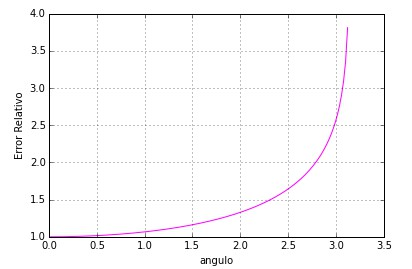
\includegraphics[width=8cm]{150.jpg}	
\caption{$n=150$}
\end{figure}

\begin{figure}[H]
	\centering
	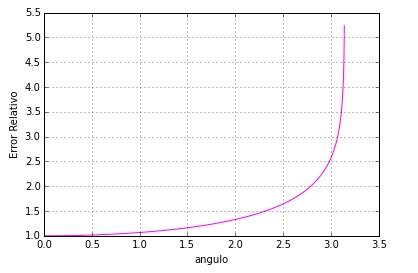
\includegraphics[width=8cm]{1000.jpg}	
	\caption{$n=1000$}
\end{figure}


\begin{thebibliography}{9}
	
	\bibitem{Wiki}
Wikipedia en Español, https://es.wikipedia.org/wiki/P%C3%A9ndulo
	\emph{Péndulo}
		\bibitem{Spicy}
	http://docs.scipy.org/doc/scipy/reference/integrate.html
	
	
		
\end{thebibliography}



\end{document}